\documentclass[10pt,conference]{IEEEtran}

\usepackage{amsmath}
\usepackage{amssymb}
\usepackage{booktabs}
\usepackage{graphicx}
\usepackage{url}
\usepackage{cite}
\usepackage{xcolor}
\usepackage{tikz}
\usetikzlibrary{arrows.meta,positioning}

\begin{document}

\title{Advisory Text Is Not Ground Truth: Reporter Coverage, Campaign
Duplication, and a Null Result for Package Naming in GHSA/OSV Malware
Advisories}

\author{\IEEEauthorblockN{Anonymous Author(s)}}

\maketitle

\begin{abstract}
Advisory databases such as GHSA and OSV are increasingly mined as ground
truth for malware behaviour in package ecosystems. We collect 401
confirmed-malicious PyPI and npm advisory records and show that they
correspond to only 200 packages and 94 independent campaigns once
cross-source re-reporting, multi-name campaigns and reporter-assigned
campaign identifiers are collapsed. We then test whether packages with
compound/generic names (e.g.\ \texttt{py-*}, \texttt{*-tools},
\texttt{*-client}) are more or less likely to have a described payload
mechanism. Pooled, the odds ratio (OR) is 0.88 [0.35, 2.21]; adjusted for
ecosystem and reporter coverage, it is 0.91 [0.33, 2.52]. The null is stable
across model specifications and across three successive versions of the
campaign grouping. Reporter coverage predicts the label far better than
naming does: reporter count and Amazon Inspector coverage each carry an OR
of 3.9--8.6 when entered alone. Reading only GHSA's text instead of the GHSA+OSV
union moves the estimate to OR 2.85 ($p=0.047$), because GHSA omits 21
mechanism descriptions that OSV carries. A human check of 51 labeler
positives found precision 0.94 [0.83, 0.98]. The naming grammar, originally
motivated by LLM package hallucination, flags only 5\% of 139 real
hallucinated names versus 16--21\% of popular benign packages, so it does
not measure hallucination-proneness. We release the frozen corpus, the
campaign-collapse method and all analysis code.
\end{abstract}

\begin{IEEEkeywords}
software supply chain, malicious packages, security advisories, PyPI, npm,
measurement validity
\end{IEEEkeywords}

% ---------------------------------------------------------------------------
\section{Introduction}
\label{sec:intro}

Malicious packages account for 49\% of vulnerability reports in npm and
14\% in PyPI~\cite{akhavani2025}, and LLM code assistants add a
new route to them: a model recommends a package that does not exist, and an
attacker registers the name~\cite{spracklen2024,huang2026}. Measurement work
on this threat increasingly treats the GitHub Security Advisory database
(GHSA) and OSV as ground truth, both for which packages are malicious and
for what the malware does.

This paper checks two assumptions that such work usually makes and rarely
tests. First, that advisory records are independent observations. They are
not: GHSA and OSV re-report the same package under different identifiers,
and one attacker squats many names with one payload. In our corpus, 401
records reduce to 94 campaigns. Second, that a mechanism mentioned in the
advisory text is a property of the malware. It is partly a property of
whoever wrote the advisory: which analysts covered a package changes
whether a mechanism is described at all. Once both are accounted for, the
association we set out to test disappears. The null result is the
consequence of measuring carefully, and we report it together with the two
corrections because both change how the next study should be designed.

\textbf{Research question.} Among confirmed-malicious packages, is
compound/generic naming associated with a described payload mechanism,
after accounting for how the advisory was reported?

\textbf{Contributions.}
\begin{enumerate}
\item A frozen, checksummed, campaign-level corpus (401 records
$\rightarrow$ 200 packages $\rightarrow$ 94 campaigns) and a reusable
two-stage collapse.
\item Evidence that mechanism labels mined from advisory text depend
strongly on reporter coverage.
\item A stable null for naming $\rightarrow$ mechanism, with a power
analysis.
\item A negative validation of a compound-naming grammar as a proxy for LLM
hallucination.
\end{enumerate}

% ---------------------------------------------------------------------------
\section{Background and Related Work}
\label{sec:related}

\textbf{Package hallucination.} Spracklen et al.~\cite{spracklen2024}
measured hallucinated package names across 16 code-generating models and
found the problem persistent across models. Churilov~\cite{churilov2026}
replicated the study on 2026 frontier models and released the set of names
hallucinated by all five models tested, which we use in
Section~\ref{sec:iv}. Huang et al.~\cite{huang2026} registered hallucinated
npm names and observed real installs, which establishes the threat model
behind this work.

\textbf{Malicious-package measurement.} Akhavani et al.~\cite{akhavani2025}
analyse vulnerability reports across ten language ecosystems and find that
malicious packages make up a large share of reported npm and PyPI
vulnerabilities. Guo et al.~\cite{guo2026} benchmark npm malicious-package
detectors on a large labelled set. Hillah et al.~\cite{hillah2026} use PyPI
registration metadata to give a calibrated posterior for
registered-but-suspicious packages. Guo et al.\ note that typosquatting
campaigns reuse identical payloads across many names, but treat each
package as a separate instance; Akhavani et al.\ remove 6,391 duplicate reports and prefer
Snyk text over GitHub advisories because it is more detailed, a
reporter-coverage choice whose effect on estimates they do not measure. We
quantify both.

\textbf{Scope.} Work on hallucinated agent-skill names that host adversarial
prompts~\cite{spira2026} concerns a different artifact and a different
mechanism, and is not studied here.

% ---------------------------------------------------------------------------
\section{Data and Method}
\label{sec:method}

\begin{figure*}[t]
\centering
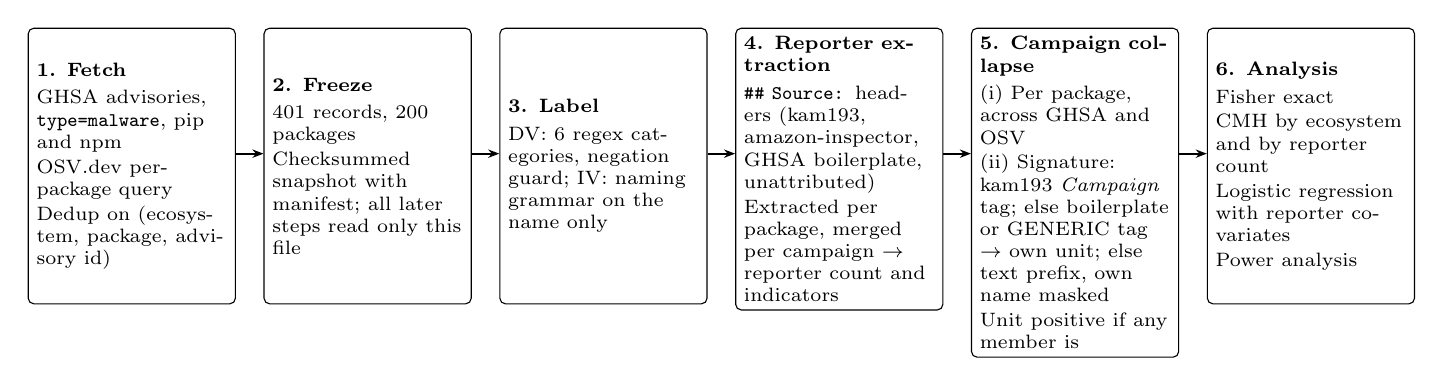
\begin{tikzpicture}[
  font=\scriptsize,
  stage/.style={draw, rounded corners=2pt, align=left, anchor=north,
                text width=2.42cm, minimum height=3.5cm, inner sep=3pt},
  arr/.style={-{Stealth[length=4pt]}, thick},
  node distance=3.5mm
]
\node[stage] (fetch) {\textbf{1. Fetch}\\[2pt]
  GHSA advisories, \texttt{type=malware}, pip and npm\\[1pt]
  OSV.dev per-package query\\[1pt]
  Dedup on (ecosystem, package, advisory id)};
\node[stage, right=of fetch.north east, anchor=north west] (freeze)
  {\textbf{2. Freeze}\\[2pt]
  401 records, 200 packages\\[1pt]
  Checksummed snapshot with manifest; all later steps read only this file};
\node[stage, right=of freeze.north east, anchor=north west] (label)
  {\textbf{3. Label}\\[2pt]
  DV: 6 regex categories, negation guard; IV: naming grammar on the name
  only};
\node[stage, right=of label.north east, anchor=north west] (reporters)
  {\textbf{4. Reporter extraction}\\[2pt]
  \texttt{\#\# Source:} headers (kam193, amazon-inspector, GHSA boilerplate,
  unattributed)\\[1pt]
  Extracted per package, merged per campaign $\rightarrow$ reporter count
  and indicators};
\node[stage, right=of reporters.north east, anchor=north west] (collapse)
  {\textbf{5. Campaign collapse}\\[2pt]
  (i) Per package, across GHSA and OSV\\[1pt]
  (ii) Signature: kam193 \emph{Campaign} tag; else boilerplate or GENERIC
  tag $\rightarrow$ own unit; else text prefix, own name masked\\[1pt]
  Unit positive if any member is};
\node[stage, right=of collapse.north east, anchor=north west] (analysis)
  {\textbf{6. Analysis}\\[2pt]
  Fisher exact\\[1pt]
  CMH by ecosystem and by reporter count\\[1pt]
  Logistic regression with reporter covariates\\[1pt]
  Power analysis};
\foreach \a/\b in {fetch/freeze, freeze/label, label/reporters,
                   reporters/collapse, collapse/analysis}
  \draw[arr] ([yshift=-1.6cm]\a.north east) -- ([yshift=-1.6cm]\b.north west);
\end{tikzpicture}
\caption{Data collection, labeling, and analysis pipeline. The DV and IV
labelers in step 3 read disjoint inputs, so the association test is not
circular.}
\label{fig:methodology}
\end{figure*}

Fig.~\ref{fig:methodology} shows the pipeline.

\subsection{Collection}
We query the GHSA API for advisories of type \texttt{malware} in the pip and
npm ecosystems and query OSV.dev for each package found. After removing
exact duplicates on (ecosystem, package, advisory id), the corpus has 401
records for 200 packages (100 per ecosystem). GHSA is a live API and
returns advisories newest first. We fetched five pages, so 386 of the 401
records were published between 1~September and 2~October 2026. The pull is
frozen to a snapshot with a SHA-256 manifest, and every number in this
paper is computed from that file.

\subsection{Campaign collapse}
\label{sec:collapse}
Fisher's and CMH tests assume independent units; without collapsing, one
npm table reached an OR of 178 on single-digit cells.

We collapse in two stages. Stage~1 merges records of the same (ecosystem,
package), which catches GHSA/OSV re-reports. Stage~2 groups packages by a
campaign signature, checked in priority order:
\begin{enumerate}
\item the reporter's own \texttt{Campaign:} identifier, when present (the
kam193 reporter assigns these);
\item otherwise the first 200 characters of the description, after
stripping \texttt{\#\# Source:} headers and masking the package's own name.
\end{enumerate}
Generic reporter templates (GHSA's ``should be considered fully
compromised'' text and kam193's generic install-time pentest template) are
never used as keys, because they are identical across unrelated incidents;
packages carrying only such text stay as their own unit. A unit counts as
grammar-flagged, or as DV-positive, if any member does. Choosing one
representative record instead silently moves campaigns between table
cells, because names within one campaign can differ in their grammar flag.

The result is 200 packages $\rightarrow$ 94 campaigns (npm 22, PyPI 72).
The npm side is dominated by a few families: two WhatsApp-library fork
families (45 and 15 names), a 10-name dependency-confusion family, and two
related families of 10 and 3 names. Together these hold 83 of the 100 npm
packages.

The human labeler check (Section~\ref{sec:dv}) found problems before it
produced a precision figure. Reading the sampled rows surfaced two grouping
failures: per-package \texttt{\#\# Source:} headers made identical texts
look different, and a 10-name family whose texts begin with the package
name was never merged. These led to the header strip and the name mask. It
also surfaced a negation false positive, ``it does not exfiltrate
credentials \ldots'', which led to the negation guard.

\subsection{Independent variable: compound/generic naming}
\label{sec:iv}
A name is flagged if it contains a token from lists of compound suffixes,
compound prefixes or trend suffixes (e.g.\ \texttt{py-}, \texttt{-tools},
\texttt{-client}, \texttt{-sdk}). The classifier reads the name only. The
grammar was designed as a proxy for names an LLM might hallucinate, so we
tested it against real hallucinations (Table~\ref{tab:grammar}). It flags
7 of the 139 names that all five models in Churilov's
study~\cite{churilov2026} hallucinated, against 16--21\% of the top-5,000
benign packages. We therefore describe the variable as compound/generic
naming, which is what it measures. The benign sets must be chosen with
care: an npm control drawn from search-API results for common terms is
flagged at 73\%, because the search terms are themselves grammar tokens.
The seven flagged hallucinated names are \texttt{aws-cdk},
\texttt{simics-6-api}, \texttt{flask-idempotency}, \texttt{aws-retry},
\texttt{rollup-plugin-es6}, \texttt{react-randomized} and
\texttt{iana-language-tag}.

\begin{table}[t]
\centering
\caption{Grammar flag rate by set, with Wilson 95\% CIs.}
\label{tab:grammar}
\begin{tabular}{lrrc}
\toprule
Set & $n$ & Flagged & Rate [95\% CI] \\
\midrule
Hallucinated names~\cite{churilov2026} & 139 & 7 & 0.050 [0.025, 0.100] \\
Benign top-5000 PyPI & 5,000 & 821 & 0.164 [0.154, 0.175] \\
Benign top-5000 npm & 5,000 & 1,031 & 0.206 [0.195, 0.218] \\
Malware campaigns & 94 & 25 & 0.266 [0.187, 0.363] \\
\bottomrule
\end{tabular}
\end{table}

\subsection{Dependent variable: described mechanism}
\label{sec:dv}
A first taxonomy, aimed at agent-directed prompt injection, found nothing:
advisory text is third-person analyst narration, not text from the package.
The dependent variable is therefore whether the advisory text describes at
least one of six mechanisms:
\begin{itemize}
\item obfuscated payload execution;
\item a hidden install hook;
\item credential or wallet exfiltration;
\item remote backdoor access;
\item remote payload retrieval;
\item a brand-impersonation narrative.
\end{itemize}
The patterns were first derived from PyPI text and flagged 0 of about 200
npm records across four pipeline runs. Adding npm phrasing
(\texttt{postinstall} hooks, JavaScript obfuscators, verbs such as
\emph{reads} and \emph{POSTs}) fixed this. A negation guard drops a match
when a cue (\emph{does not}, \emph{do not}, \emph{did not},
\emph{doesn't}, \emph{no evidence of}) occurs within 40 characters before
it, unless \emph{but}, a semicolon or a period intervenes. The labeler's
signature accepts text only, never the name, and a test enforces this.

The text is the union of a package's GHSA and OSV descriptions. Under this
setting, 21 packages are positive only because of text that OSV carries and
GHSA omits: 20 through an amazon-inspector section and one through a kam193
section. On reading, all 21 describe real mechanisms. GHSA-only text is
reported as a sensitivity analysis (Section~\ref{sec:ghsa}).

One author annotated 51 labeler positives under a written rule: all 21
OSV-only positives, plus 30 sampled campaigns (an npm census of 12 and a
seeded draw of 18 PyPI). Matches found only in analyst tag lists, not in
prose, count as FALSE. The result was 44 REAL, 3 FALSE and 4 UNSURE, giving
precision 0.936 [0.828, 0.978] excluding UNSURE and 0.863 [0.743, 0.932]
counting UNSURE as FALSE. All 3 FALSE rows were tag-line-only matches, and
2 of them contain prose describing the behaviour that the regex missed, so
as a measure of label correctness these figures are conservative.
Annotators saw package names, and recall was not measured.

\subsection{Reporter coverage}
We parse the \texttt{\#\# Source:} headers in both texts of every package
and merge them per campaign. GHSA's boilerplate and OSV's
\texttt{ghsa-malware} section are the same text and count as one reporter.
Headerless text without boilerplate is \emph{unattributed} (73 of 200
packages). From the parsed headers we derive a reporter count
(\texttt{n\_reporters}) and three indicators: kam193, amazon-inspector and
boilerplate.

\subsection{Analysis}
\label{sec:analysis}
We use Fisher's exact test on the pooled and per-ecosystem $2\times2$
tables, and CMH tests stratified by ecosystem and by ecosystem $\times$
reporter count~\cite{agresti}. We fit the logistic regression
$\mathit{DV} \sim \mathit{grammar} + \mathit{ecosystem} +
\mathit{n\_reporters} + \mathit{amazon\_inspector}$ (model~d), and three
variants: (a)~without the Amazon term, (b)~without the reporter count, and
(c)~(a) plus the boilerplate and kam193 indicators. ORs come with Woolf,
Robins--Breslow--Greenland or Wald 95\% CIs as appropriate. Power at the
achieved $n$ follows Hsieh et al.~\cite{hsieh1998}.

% ---------------------------------------------------------------------------
\section{Results}
\label{sec:results}

\subsection{Descriptive}
Of the 94 campaigns, 25 are grammar-flagged and 51 are DV-positive. The DV
rate depends strongly on who reported the campaign:
\begin{itemize}
\item amazon-inspector coverage: 0.65 (46/71), against 0.22 (5/23)
without;
\item kam193 coverage: 0.59 (37/63);
\item boilerplate among the reporters: 0.38 (5/13); boilerplate as sole reporter: 0/4.
\end{itemize}
Reporter coverage is not independent of naming either. The GHSA boilerplate
appears in 0 of 74 records of flagged packages, against 26 of 327 records
of unflagged packages.

\begin{table*}[t]
\centering
\caption{Grammar flag vs.\ described mechanism, 94 campaigns, GHSA+OSV
text unless noted. Regression models (a)--(d) as defined in
Section~\ref{sec:analysis}.}
\label{tab:main}
\begin{tabular}{llcclc}
\toprule
Specification & $n$ & Grammar OR [95\% CI] & $p$ & Reporter terms, OR [95\% CI] & $p$ \\
\midrule
Pooled, Fisher & 94 & 0.884 [0.353, 2.211] & 0.818 & & \\
npm, Fisher & 22 & 2.200 [0.323, 14.975] & 0.624 & & \\
PyPI, Fisher & 72 & 0.673 [0.234, 1.940] & 0.587 & & \\
CMH by ecosystem & 94 & 0.890 [0.355, 2.232] & 0.802 & & \\
CMH by ecosystem $\times$ reporter count & 94 & 1.067 [0.402, 2.830] & 0.891 & & \\
\midrule
Logit (d) & 94 & 0.912 [0.331, 2.515] & 0.858 & n\_reporters 1.862 [0.528, 6.568] & 0.334 \\
 & & & & amazon-inspector 3.388 [0.701, 16.372] & 0.129 \\
Logit (a) & 94 & 0.992 [0.360, 2.732] & 0.987 & n\_reporters 3.898 [1.572, 9.664] & 0.003 \\
Logit (b) & 94 & 0.855 [0.317, 2.310] & 0.758 & amazon-inspector 5.857 [1.898, 18.073] & 0.002 \\
Logit (c) & 94 & 0.827 [0.279, 2.448] & 0.731 & n\_reporters 8.623 [2.316, 32.098] & 0.001 \\
 & & & & boilerplate 0.211 [0.022, 2.070] & 0.182 \\
 & & & & kam193 0.158 [0.024, 1.030] & 0.054 \\
\midrule
\emph{Sensitivity: GHSA text only, Fisher} & 94 & 2.851 [1.107, 7.341] & 0.047 & & \\
\bottomrule
\end{tabular}
\end{table*}

\subsection{Main test}
The pooled table is $[[13,12],[38,31]]$, which gives OR 0.884 [0.353,
2.211], $p=0.818$ (Table~\ref{tab:main}). Adjusting for ecosystem with CMH
gives 0.890 [0.355, 2.232], $p=0.802$. The npm stratum ($n=22$) is too
small to interpret on its own.

\subsection{Adjusted}
In model~(d) the grammar OR is 0.912 [0.331, 2.515], $p=0.858$. Reporter coverage explains the
label instead. Entered without its collinear partner, the reporter count
has OR 3.90 (model~a) and Amazon Inspector coverage OR 5.86 (model~b), both
$p\le0.003$. With both terms in the model (variance inflation factors 2.3),
neither is individually significant, but model~(d) as a whole is
(likelihood-ratio $p=0.0036$). The grammar flag's variance inflation factor
is 1.01.

\subsection{Text-source sensitivity}
\label{sec:ghsa}
Reading only GHSA's text gives OR 2.851 [1.107, 7.341], $p=0.047$ (CMH
2.907, $p=0.023$). We do not treat this as a finding, for four reasons:
\begin{itemize}
\item It is one of many text, grouping and signature settings we examined,
with no correction for multiple comparisons.
\item Its npm stratum has a zero cell: none of the 16 unflagged npm
campaigns is DV-positive under GHSA text.
\item The regression with boilerplate and kam193 terms does not converge,
because no boilerplate campaign is DV-positive under GHSA text.
\item The gap is explained by reporter coverage. None of the 21 packages
that are positive only through OSV-carried text is grammar-flagged, against
37 of the other 179 packages (Fisher $p=0.016$).
\end{itemize}
A single-source estimate is therefore not ``cleaner''; it is biased by
which reporter's text was dropped.

\subsection{Power}
With 26.6\% of campaigns flagged and a baseline DV rate of 0.55 among
unflagged campaigns, the design has 0.31 power at OR 2.0 and 0.65 at OR 3.0.
Reaching 80\% power at OR 2.0 needs about 339 campaigns.

% ---------------------------------------------------------------------------
\section{Discussion}
\label{sec:discussion}

\textbf{What the null means.} We find no evidence that compound/generic
naming goes with a described mechanism. At $n=94$ this rules out only large
effects (OR $\gtrsim 3$); it is not evidence that no effect exists. A
cost-minimising attacker model~\cite{allodi2022} could still motivate a
directional hypothesis for a larger study, but it cannot explain a result
we did not observe.

\textbf{What the reporter finding means for others.} Any study that uses
GHSA or OSV text as a behavioural label inherits a reporter-coverage
confound. Dropping one source changed our estimate from 0.88 to 2.85,
because the dropped reporter's detail went disproportionately to unflagged
packages. We recommend three practices:
\begin{itemize}
\item use the union of the source texts;
\item parse reporter sections;
\item control for reporter count.
\end{itemize}

\textbf{Why we do not claim ``sophistication''.} The dependent variable is
whether any mechanism is described. A count of distinct categories shows no
difference either: a mean of 0.76 for flagged and 0.70 for unflagged
campaigns (Mann--Whitney $p=0.92$).

\textbf{Why we do not claim ``hallucination''.} The grammar flags 5\% of
real hallucinations, most of which are import or module names used as
package names (\texttt{objc}, \texttt{opentelemetry},
\texttt{tencentcloud}), so it measures generic naming. The gradient from
16--21\% (benign) to 27\% (malware campaigns) is descriptive, and the sets
are not matched.

\textbf{Ecosystems.} The npm stratum consists of a handful of families plus
singletons, so this study supports no per-ecosystem claim.

% ---------------------------------------------------------------------------
\section{Threats to Validity}
\label{sec:threats}

\textbf{Construct.} The labeler is a regex taxonomy. Its check is a
single-annotator review of 51 positives (precision 0.94 [0.83, 0.98]), with
no inter-annotator agreement and no recall estimate. The grammar is
validated only as a measure of generic naming.

\textbf{Internal.} Reporter coverage is modelled but not exhausted:
37\% of packages are unattributed. As superseded history, the campaign
grouping changed three times during the study (142 $\rightarrow$ 106
$\rightarrow$ 94 campaigns) as the labeler check surfaced merge failures,
and further under-merging is possible. The point estimate crossed 1 across
those changes (0.85, 1.18, 0.88), which itself suggests there is no signal
at this $n$.

\textbf{External.} The corpus covers a five-week window, two ecosystems and
94 campaigns. Of these, 22 are npm campaigns dominated by a few families.

\textbf{Statistical.} The study is underpowered for OR $<3$, several strata
are sparse, and CMH assumes a homogeneous OR across strata.

% ---------------------------------------------------------------------------
\section{Conclusion and Future Work}
\label{sec:conclusion}

Advisory records are not independent, and advisory text is not ground
truth. After correcting for both, compound/generic naming shows no
association with described malware mechanisms, while reporter coverage
does. Next steps:
\begin{itemize}
\item grow the corpus backward in time to about 350 campaigns;
\item validate the labeler with two annotators and add a matched benign
comparison;
\item build a hallucination instrument based on import names rather than
naming grammar.
\end{itemize}

\textbf{Artifact availability.} The frozen snapshot, manifests, analysis
code and tests are available at [anonymized]. GHSA advisory data are
licensed CC BY 4.0, OSV records carry per-source licences, and the
hallucinated-name set~\cite{churilov2026} is CC BY 4.0.

\section*{Acknowledgments}
The authors used an AI assistant (Claude, Anthropic) for help with code
and drafting. The authors reviewed all code, analyses and text and take
full responsibility for the content of this paper.

\IEEEtriggeratref{2}
\begin{thebibliography}{10}

\bibitem{spracklen2024}
J.~Spracklen, R.~Wijewickrama, A.~H.~M.~N.~Sakib, A.~Maiti, B.~Viswanath, and M.~Jadliwala, ``We have a package for you! A comprehensive analysis of package hallucinations by code generating LLMs,'' in \textit{Proc. 34th USENIX Security Symposium}, 2025, arXiv:2406.10279.

\bibitem{spira2026}
A.~Spira, S.~Cohen, E.~Feldman, R.~Bitton, A.~Wool, and B.~Nassi, ``Beware of agentic botnets: Scalable untargeted promptware attacks via universal and transferable adversarial HalluSquatting,'' \textit{arXiv preprint arXiv:2607.07433}, 2026.

\bibitem{hillah2026}
L.~M.~Hillah, J.-M.~Richard, and R.~Hasnaoui, ``Bayesian-calibrated detection of hallucinated package imports in AI-assisted code,'' \textit{arXiv preprint arXiv:2606.13918}, 2026.

% TODO camera-ready: add DOI
\bibitem{huang2026}
Z.~Huang, C.~Liu, Z.~Wang, X.~Cui, X.~Deng, and M.~Xu, ``Package hallucinations as phantoms in open-source software supply chains: An empirical security analysis,'' \textit{ACM Trans. Softw. Eng. Methodol.}, 2026.

\bibitem{allodi2022}
L.~Allodi, F.~Massacci, and J.~Williams, ``The work-averse cyberattacker model: Theory and evidence from two million attack signatures,'' \textit{Risk Analysis}, vol.~42, no.~8, pp.~1623--1642, 2022.

\bibitem{agresti}
A.~Agresti, \textit{Categorical Data Analysis}, 3rd ed. Hoboken, NJ, USA: Wiley, 2013.

\bibitem{hsieh1998}
F.~Y.~Hsieh, D.~A.~Bloch, and M.~D.~Larsen, ``A simple method of sample size calculation for linear and logistic regression,'' \textit{Statistics in Medicine}, vol.~17, no.~14, pp.~1623--1634, 1998.

\bibitem{churilov2026}
A.~Churilov, ``The range shrinks, the threat remains: Re-evaluating LLM package hallucinations on the 2026 frontier-model cohort,'' \textit{arXiv preprint arXiv:2605.17062}, 2026.

\bibitem{guo2026}
W.~Guo, Z.~Chen, Z.~Xu, C.~Liu, M.~Kang, S.~Song, C.~Liu, Y.~Xu, W.~Sun, and Y.~Liu, ``How effective are NPM malicious package detectors? A large-scale empirical study,'' \textit{arXiv preprint arXiv:2603.27549}, 2026.

\bibitem{akhavani2025}
S.~A.~Akhavani, B.~Ousat, and A.~Kharraz, ``Open source, open threats? Investigating security challenges in open-source software,'' \textit{arXiv preprint arXiv:2506.12995}, 2025.

\end{thebibliography}

\end{document}
